% differential drive robot math
\documentclass[11pt]{article}

\usepackage{ebgaramond}
\usepackage[T1]{fontenc}
\usepackage{graphicx}
\usepackage{amsmath}

\usepackage{url}


\usepackage{listings}
\usepackage{color}

\definecolor{dkgreen}{rgb}{0,0.6,0}
\definecolor{gray}{rgb}{0.5,0.5,0.5}
\definecolor{mauve}{rgb}{0.58,0,0.82}

\lstset{frame=tb,
  language=Python,
  aboveskip=3mm,
  belowskip=3mm,
  showstringspaces=false,
  columns=flexible,
  basicstyle={\small\ttfamily},
  numbers=none,
  numberstyle=\tiny\color{gray},
  keywordstyle=\color{blue},
  commentstyle=\color{dkgreen},
  stringstyle=\color{mauve},
  breaklines=true,
  breakatwhitespace=true,
  tabsize=3
}

\title{The Kinematics of a Differential Drive Robot}
\author{Iain Brookshaw}

\begin{document}
\maketitle
\begin{abstract}
    Non-holonomic\footnote{Non-holonomic: in this context, a vehicle that may move in one less dimension than the 
    system possesses. eg: a car can rotate and move forward, but not "crab" sideways.}, differential drive robots are 
    the basis of most mobile robotics; the platform is simple, robust and readily adaptable
    to most indoor applications.

    The kinematics of such platforms is the computation of the location of the robot's base
    from an arbitrary starting point or origin frame; and is an essential step in localizing the robot.
    This document provides an exact solution for 2D differential-drive robot kinematics and is intended as a reference.
\end{abstract}

\section{Introduction}

A differential drive robot has two wheels connected along a common axis to a rigid chassis, with a un-powered castor
or ball-bearing providing a third point of floor contact. It may thus rotate and drive forwards and backwards, but 
cannot move sideways.

Each wheel can be controlled  independently and has an encoder attached to the motor drive shaft, allowing accurate 
measurement of the wheel's rotational velocity. Using this value, the known radius of the wheel, the known motor 
\& gearbox ratio and assuming there is no wheel slip, the linear speed of each wheel ($v_r$ and $v_l$) can be
calculated in meters per second\footnote{The lack of slip assumption is the critical and most often violated 
assumption in this method.}.

In these calculations, we are computing the new {\em pose} $[x',y',\theta']$ of the robot at some time $\delta t$ after
the original pose $[x,y,\theta]$. In both cases $x,y$ and $\theta$ are in world coordinates, with $\theta$ being the 
angle from the global $X$ axis to the robot's local heading (see Figure \ref{robot}).

\begin{figure}
    \centering
    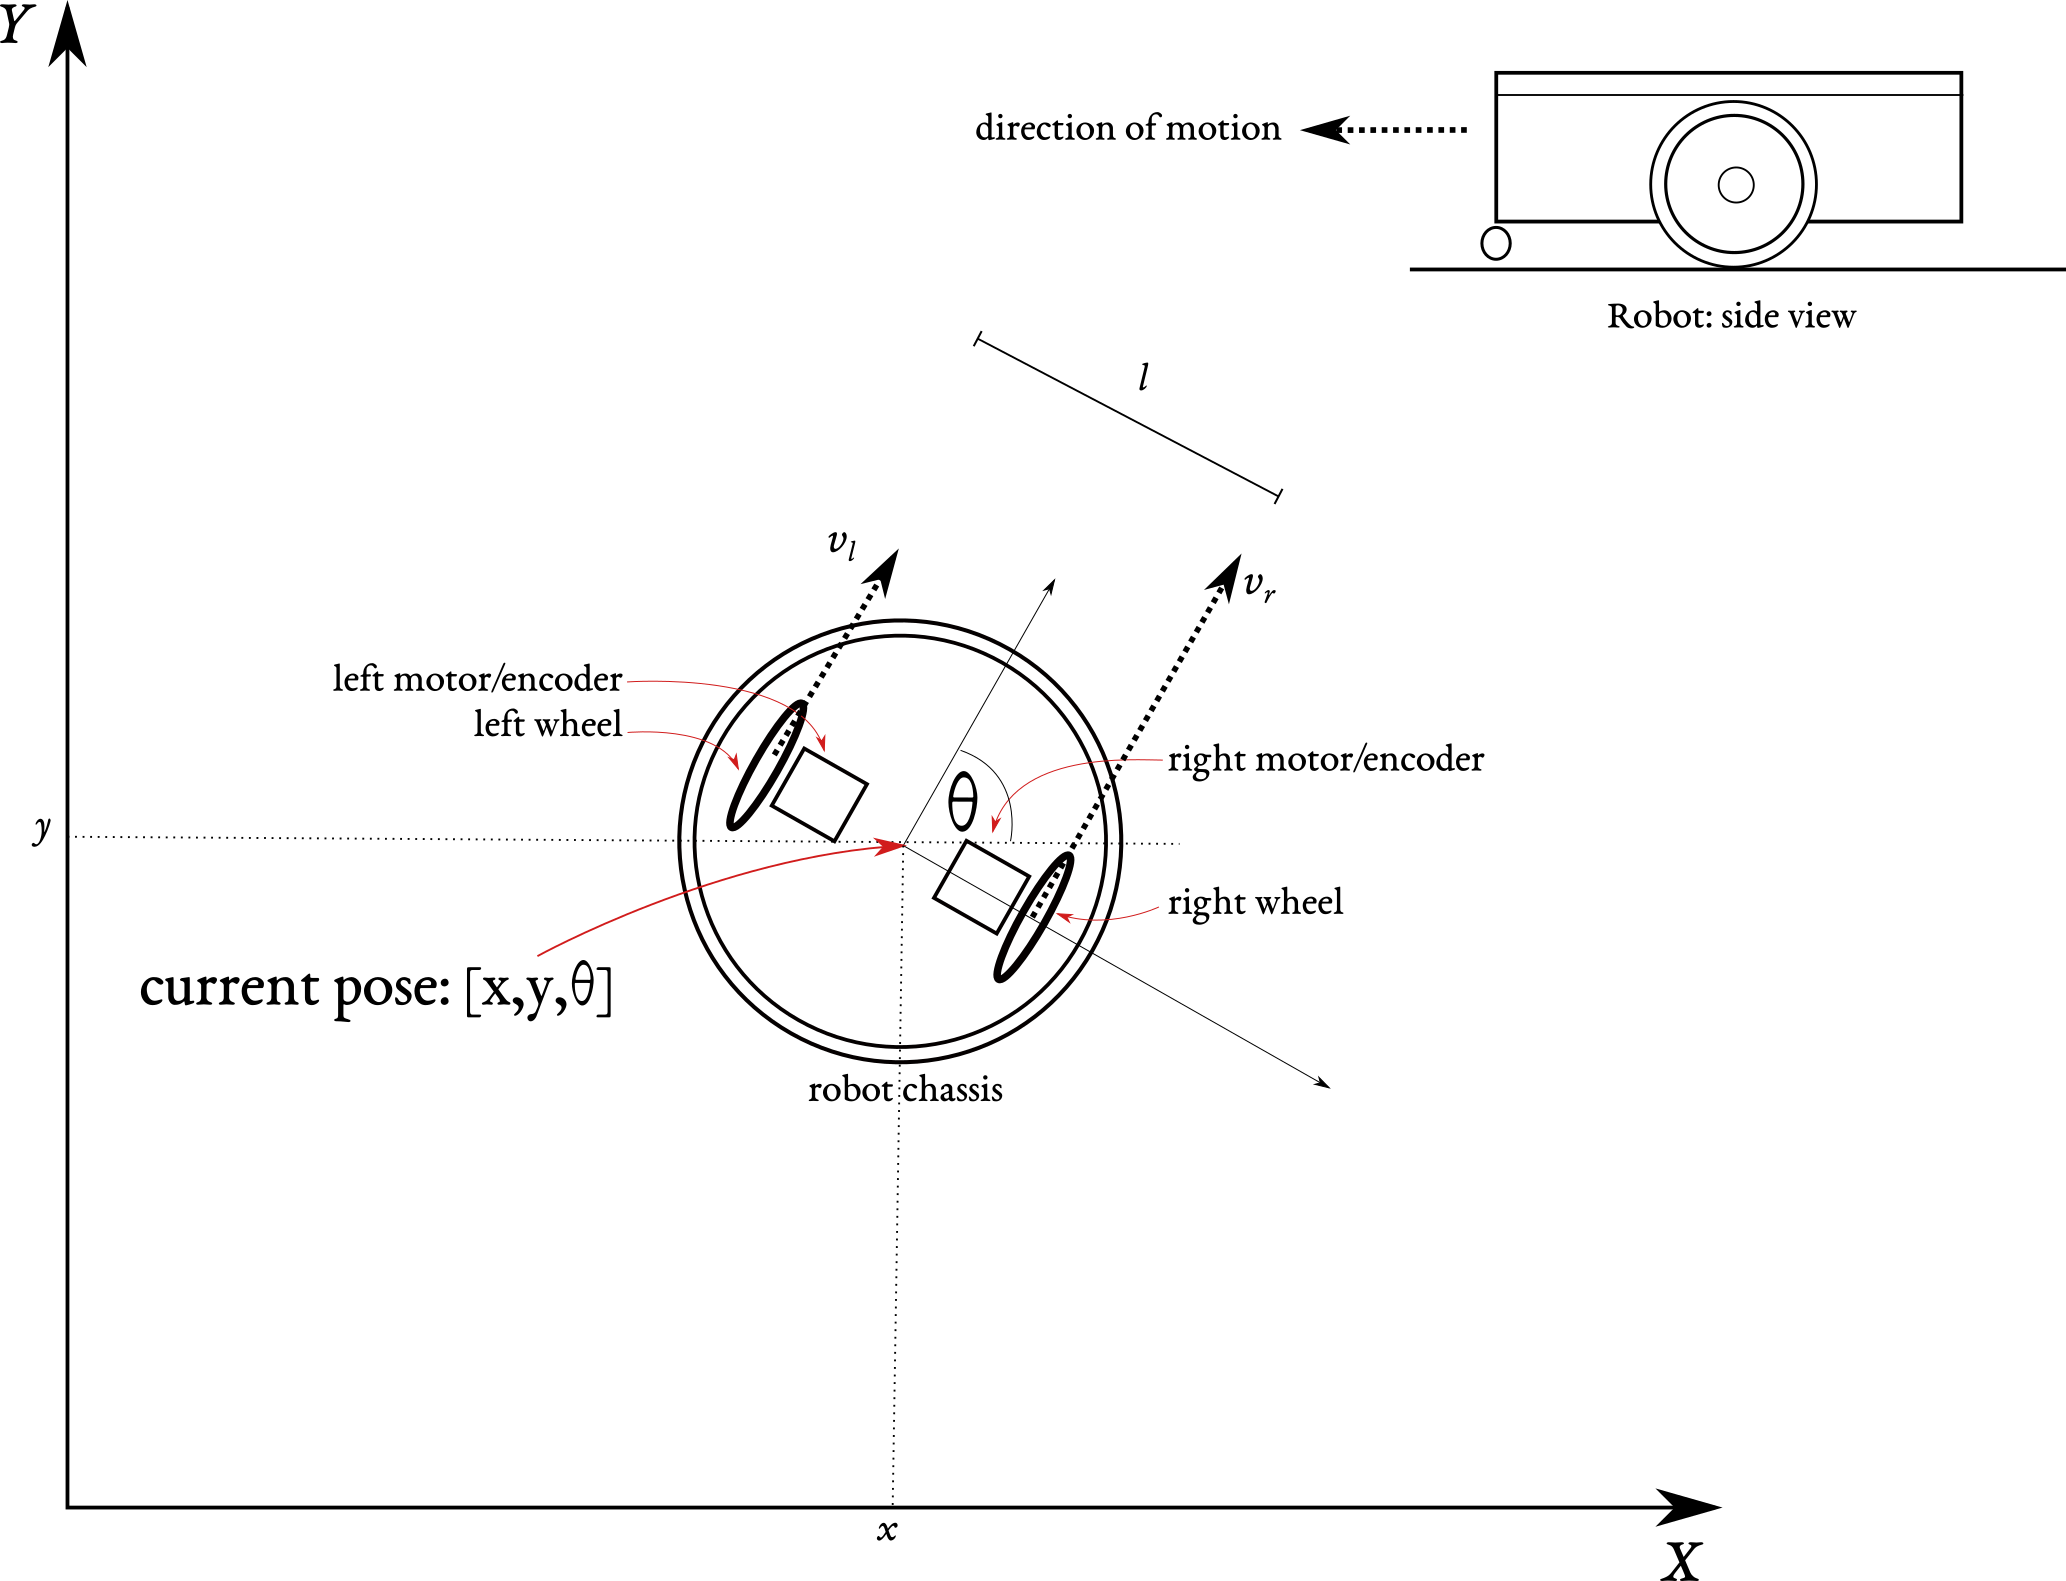
\includegraphics[width=0.8\textwidth]{images/robot.png}
    \caption{The differential drive robot, showing the robot pose $[x,y,\theta]$, the left and right wheel velocities 
             ($v_l$ and $v_r$), the wheelbase ($l$), the heading ($\theta$) and the local and global coordinate frames}
    \label{robot}
\end{figure}

If these wheel velocities are equal (or approximately equal to a given acceptable step error $\epsilon$), then the new position
is simply\footnote{As they are equal, either $v_l$ or $v_r$ can be used here}:
\begin{eqnarray}
    x' &=& x + v_l / \delta t \\
    y' &=& y + v_l / \delta t \\
    \theta' &=& \theta
\end{eqnarray}

However, if the robot is rotating as well as moving forwards, a more sophisticated approach is needed.

\section{Derivation}

Because the robot is rigid, both wheels rotate around a common point of rotation, the "Instantaneous Center of Curvature" 
($ICC$) at the same rotational speed ($\omega$ rad/sec). The $ICC$ exists along a line of length $R$ through the center
of both wheels (see Figure \ref{fig:arc}). This $R$ value is constant for both poses of the robot.

\begin{figure}
    \centering
    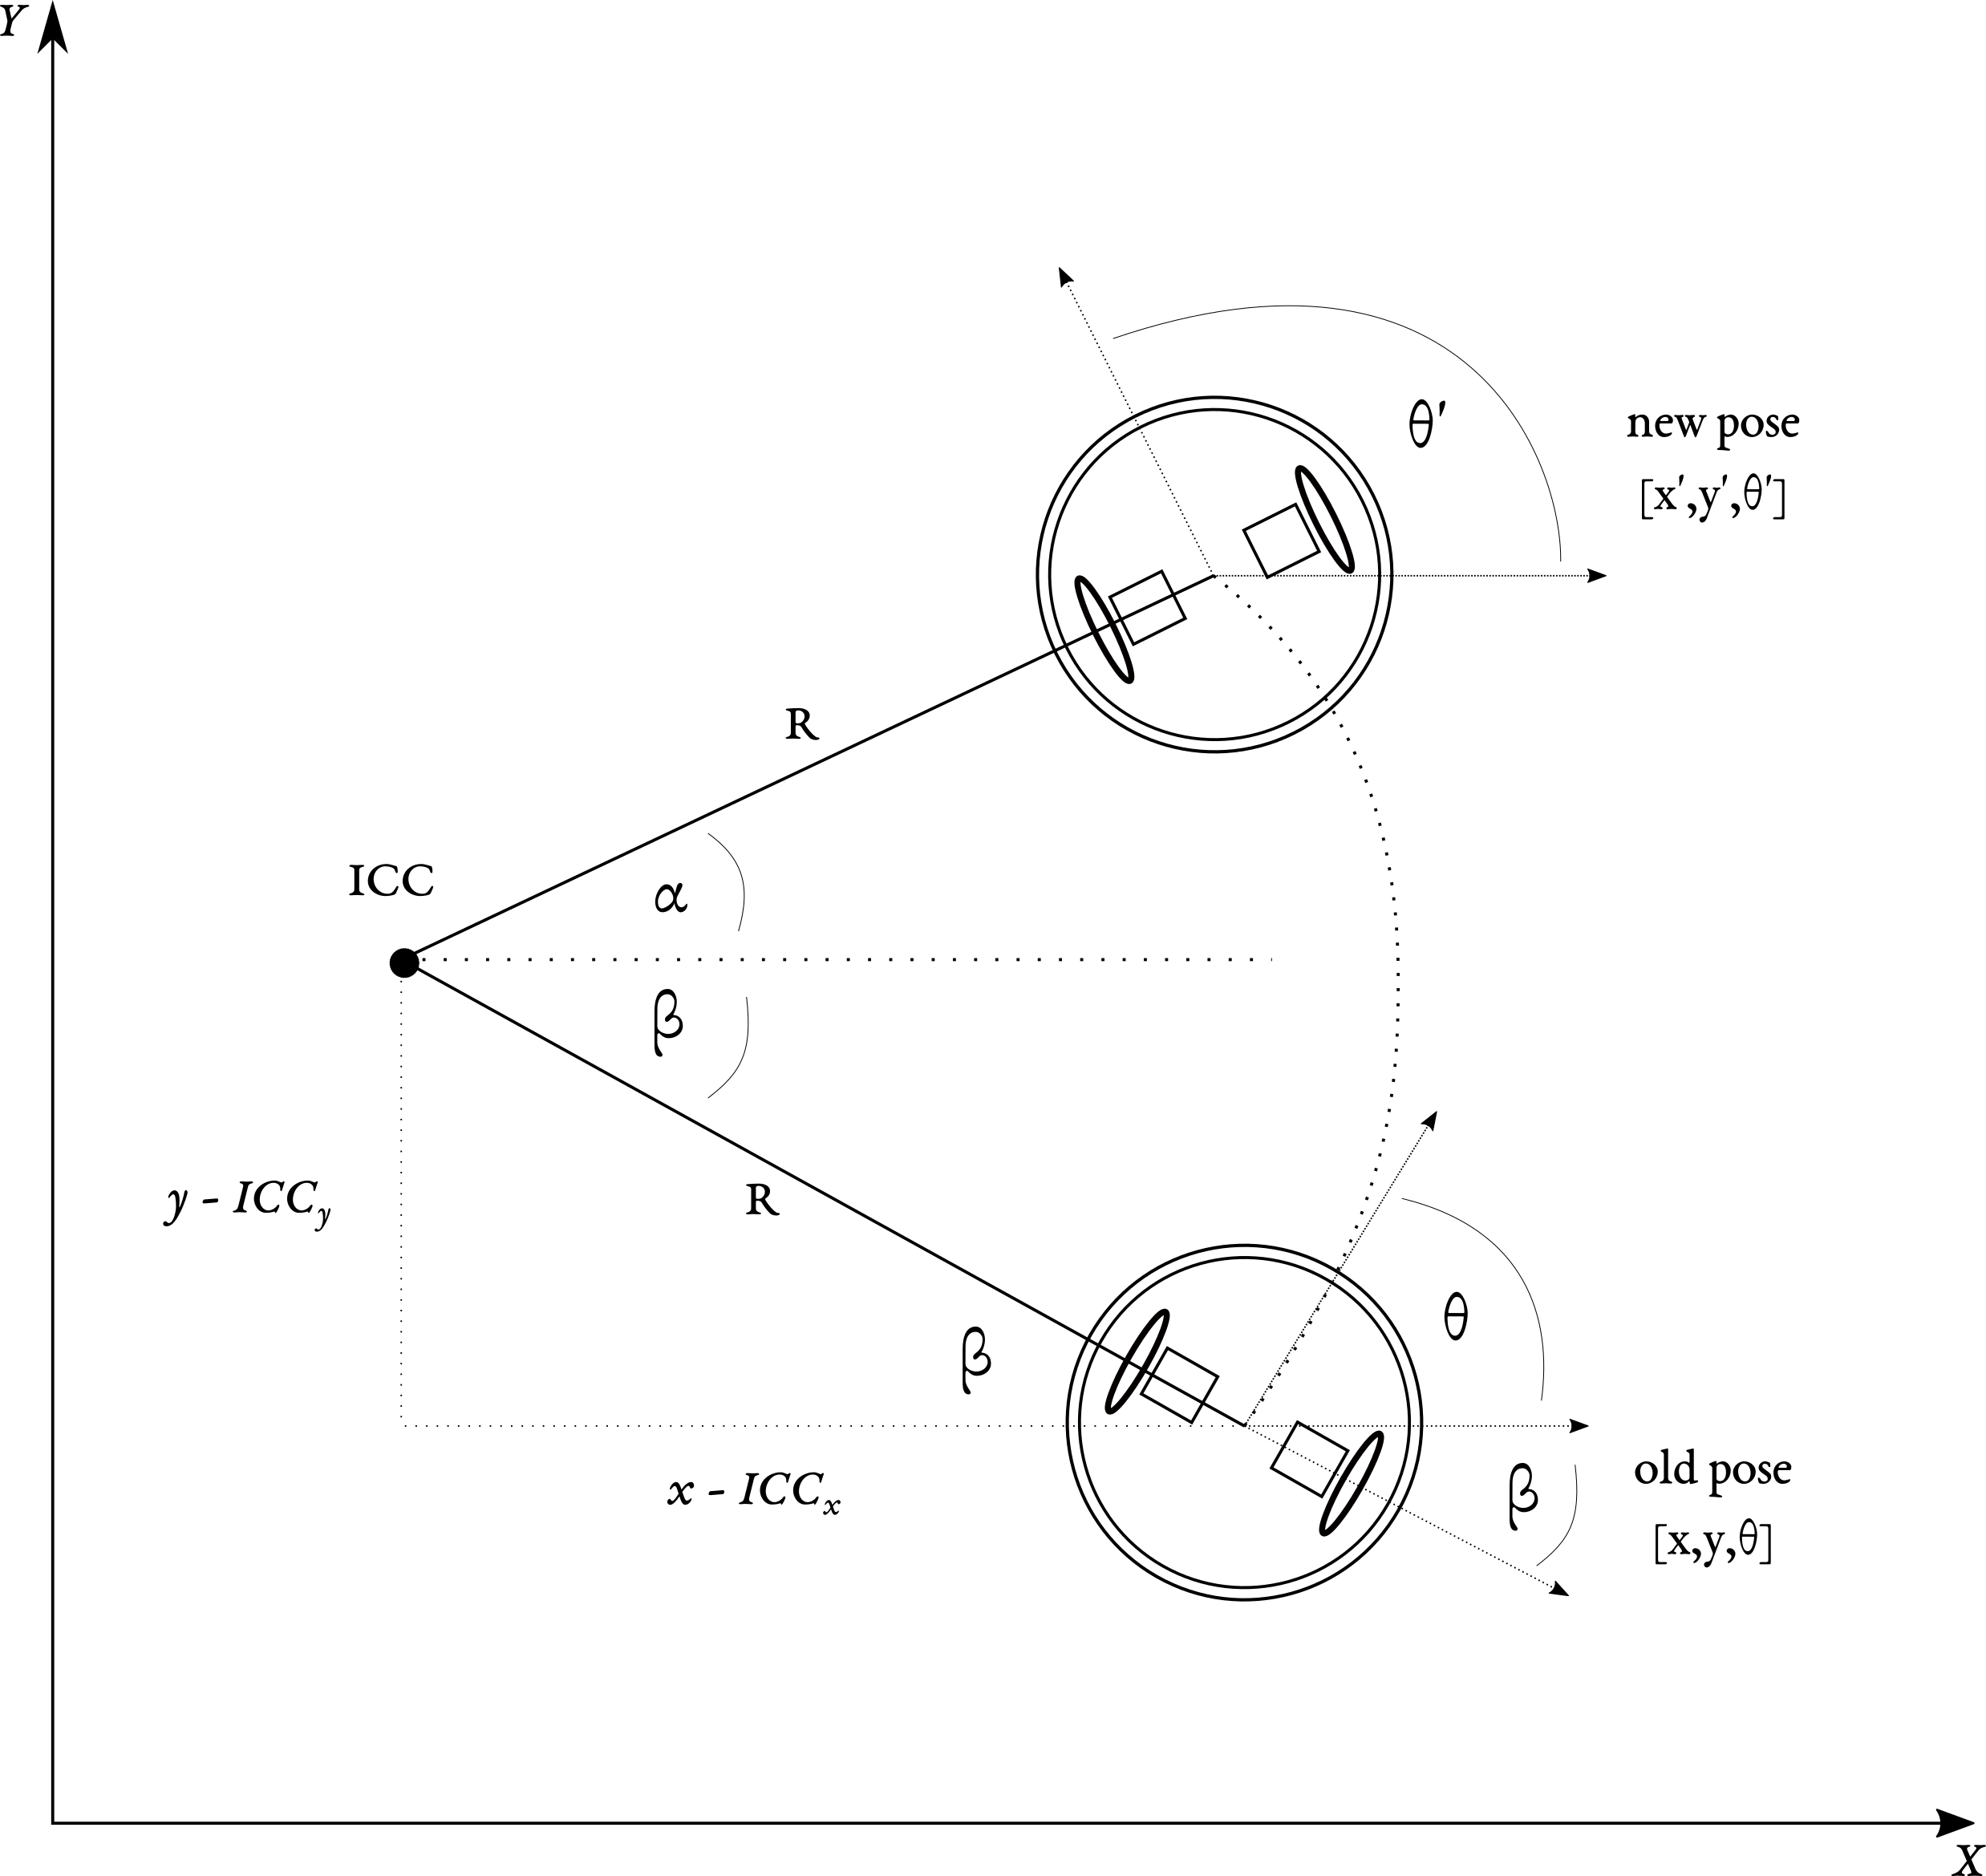
\includegraphics[width=0.8\textwidth]{images/arc.png}
    \caption{The robot rotation over $\delta t$, showing the $ICC$, the angles $\alpha$ and $\beta$ and the 
             radius of rotation $R$}
    \label{fig:arc}
\end{figure}

From this we can see that $\omega\times r = v$, where $v$ is the velocity at any point $r$ on the line $R$. As we know 
the velocity at the wheels, we can produce two equations for these two unknowns:
\begin{eqnarray}
    \omega(R + l/2) &=& v_r \label{eqn:w_vr} \\
    \omega(R - l/2) &=& v_l \label{eqn:w_vl}
\end{eqnarray}

Rearranging equations \ref{eqn:w_vr} and \ref{eqn:w_vl} gives us the following results for $R$ and $\omega$:

\begin{eqnarray}
    R &=& \frac{\frac{l}{2}(v_l + v_r)}{v_r - v_l} \label{eqn:R} \\
    \omega &=& \frac{v_r - v_l}{l} \label{eqn:w}
\end{eqnarray}

Thus $R$ and $\omega$ are now known.

\subsection{Computing The New Heading}

\begin{figure}
    \centering
    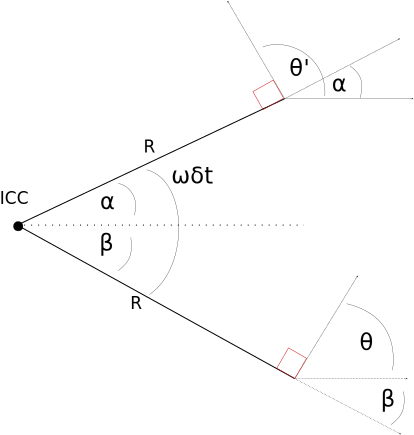
\includegraphics[width=0.8\textwidth]{images/theta-proof}
    \caption{Illustration of the computation of the computation of $\theta'$, showing the relationship between 
    $\alpha$, $\beta$, $\theta$ and $\theta'$ for a robot moving around $ICC$.}
    \label{fig:theta-proof}
\end{figure}

Figure \ref{fig:arc} shows that the angle around the $ICC$ from current pose $ = [x,y,\theta]$ to new pose $ = [x',y',\theta']$ is 
$\omega\delta t$, where $\delta t$ is the known time difference between the two poses. From this, we can deduce that
$\theta'$ is:
\begin{equation}
    \theta' = \theta + \omega\delta t \label{eqn:theta}
\end{equation}

We can prove this as follows:

As can be seen in Figure \ref{fig:theta-proof}: 
\begin{equation}
    \alpha + \beta = \omega\delta t
\end{equation}
Therefore, through similar triangles:
\begin{eqnarray}
    \theta' - \alpha &=& \pi/2 \nonumber\\   
    \theta + \beta &=& \pi/2 
\end{eqnarray}
Thus we can solve for $\theta'$:
\begin{eqnarray}
\theta' &=& \theta + \beta + \alpha \nonumber\\
\theta' &=& \theta + \omega\delta t
\end{eqnarray}
All of which are now known quantities.


To compute the remainder of the pose, we first need to compute the position of $ICC$ in world coordinates.

\subsection{Computing The New Pose}

As can be seen in Figure \ref{fig:theta-proof}, the line $R$ forms the hypotenuse of a right-angle triangle 
with $ICC$ and the old pose at $[x,y,\theta]$ (see Figure \ref{fig:arc})
From this, we can deduce the following equations:

\begin{eqnarray}
R\cos{\beta} &=& x - ICC_x \label{eqn:Rcos}\\
R\sin{\beta} &=& y - ICC_y \label{eqn:Rsin}
\end{eqnarray}

By recalling that $\beta + \alpha = \omega\delta t$ and by observing that $\theta + \beta = \pi/2$, we can express
equations \ref{eqn:Rcos} and \ref{eqn:Rsin} in terms of $\theta$ thus:

\begin{eqnarray}
R\cos(\theta - \pi/2) &=& x -ICC_x \\ 
R\sin(\theta - \pi/2) &=& y -ICC_y
\end{eqnarray}

By recalling the following trig-identities:
\begin{eqnarray} 
    \cos{a-b} &=& \cos{a}\cos{b} + \sin{a}\sin{b} \nonumber \\
    \sin{a-b} &=& \sin{a}\cos{b} - \sin{b}\cos{a} \nonumber
\end{eqnarray}
and that:
\begin{eqnarray}
    \cos{\pi/2} &=& 0 \nonumber \\
    \sin{\pi/2} &=& 1 \nonumber 
\end{eqnarray}
we can solve for $[ICC_x, ICC_y]$:

\begin{eqnarray}
    ICC_x = x - R\sin{\theta} \label{eqn:icc-x} \\
    ICC_x = y + R\sin{\theta} \label{eqn:icc-y} \\
\end{eqnarray}

To reach the new pose, we are rotating around $ICC$ at a radius of $R$ and through an angle $\omega\delta t$. All of these
quantities are now known, thus a standard rotation matrix gives us the new pose (for notational simplicity, let 
$\gamma = \omega\delta t$):

\begin{equation}
\begin{bmatrix}x'\\y'\end{bmatrix} = %
\begin{bmatrix}
c_{\gamma} & -s_{\gamma} \\
s_{\gamma} &  c_{\gamma}
\end{bmatrix}
\begin{bmatrix}
x - ICC_x \\
y - ICC_y
\end{bmatrix} +
\begin{bmatrix}
ICC_x\\
ICC_y
\end{bmatrix}
\label{eqn:new-pose}
\end{equation}

Equation \ref{eqn:new-pose} gives the position of the robot in world coordinates $\delta t$ seconds after the last position
computation. This is repeated as necessary to provide the ongoing position of the robot.

% ======================================================================================================================
\newpage
\appendix
\section{Algorithm}

To solve this numerically, we would need to implement the following psudo-code:
\begin{lstlisting}

def update_pose( v_l, v_r, epsilon, delta_t, old_pose ):
    """
    Compute the new pose of the robot from the motor movement
    :param v_l: float - linear velocity of left wheel (m/s)
    :param v_r: float - linear velocity of right wheel (m/s)
    :param epsilon: float - float comparator constant (m/s)
    :param delta_t: float - time step from last update to this (s)
    :param old_pose: tuple (x,y,theta) last update pose (m,m,rad)
    :returns: tuple (x',y',theta') new pose (m,m,rad)
    """

    # do simple case of straight line first
    if _compare_v(v_l, v_r, epsilon):
        return (
            old_pose.y,
            old_pose.x + v_l*delta_t,
            old_pose.theta )

    # now do more complex, rotation around ICC case
    R   = _compute_r(v_l, v_r)
    w   = _compute_omega(v_l, v_r)
    ICC = _compute_icc(R, old_pose)

    new_theta = _compute_new_theta(
        old_pose,
        omega,
        delta_t)

    new_x, new_y = _compute_new_coordinate(
        old_pose, 
        omega, 
        delta_t, 
        ICC)

    return (
        new_x,
        new_y,
        new_theta )
\end{lstlisting}


\section{Variables}

    \begin{tabular}{c p{8cm}}
        $[x, y, \theta]$ & Original pose at time = 0 seconds in global coordinates (meters) and the heading of the robot (radians) \\
        $[x', y', \theta']$ & Final pose at time = $\delta t$ seconds in global coordinates (meters) and the heading of the robot (radians) \\
        $l$ & The robot's wheelbase in meters \\
        $v_l$ & The scalar linear velocity of the left wheel of the robot (meters/second) \\
        $v_r$ & The scalar linear velocity of the right wheel of the robot (meters/second) \\ 
        $ICC$ & The Instantaneous Center of Curvature -- the point in world coordinates around which the robot is rotating \\
        $\omega$ & The rotational velocity around the $ICC$ in radians/second \\
        $R$ & The distance from the $ICC$ to the robot (meters). This is constant at both time=0 and time=$\delta t$\\
        $\gamma$ & The angle the robot rotates around $ICC$, given by $\omega\delta t$ in radians
    \end{tabular}

% ======================================================================================================================
\begin{thebibliography}{10}
\bibitem{DudekJenkin}
\url{http://www.cs.columbia.edu/~allen/F17/NOTES/icckinematics.pdf}

\bibitem{Hellstrom}
\url{http://www8.cs.umu.se/kurser/5DV122/HT13/material/Hellstrom-ForwardKinematics.pdf}

\bibitem{Christensen}
\url{https://www.cc.gatech.edu/~dellaert/07F-Robotics/Schedule_files/04-Kinematics.pdf}
\end{thebibliography}

\end{document}